
\section{Separación de responsabilidades}

El sistema completo debe resolver problemas de naturaleza diferente.
Por un lado, debe observar una entrada asíncrona y reconstruir una
trama UART bit a bit; por otro, debe conservar bytes mientras los
bloques avanzan a ritmos distintos, reconocer el orden A--B--opcode,
ejecutar la operación y volver a serializar el resultado. Reunir esas
tareas en un único módulo mezclaría tiempos de bit, reglas del
protocolo y cálculo aritmético. Por eso el diseño elegido distribuye el
trabajo entre módulos con interfaces explícitas.

La figura~\ref{fig:arquitectura-general} presenta la arquitectura general y el
recorrido completo de una operación.

\begin{figure}[H]
 \centering
 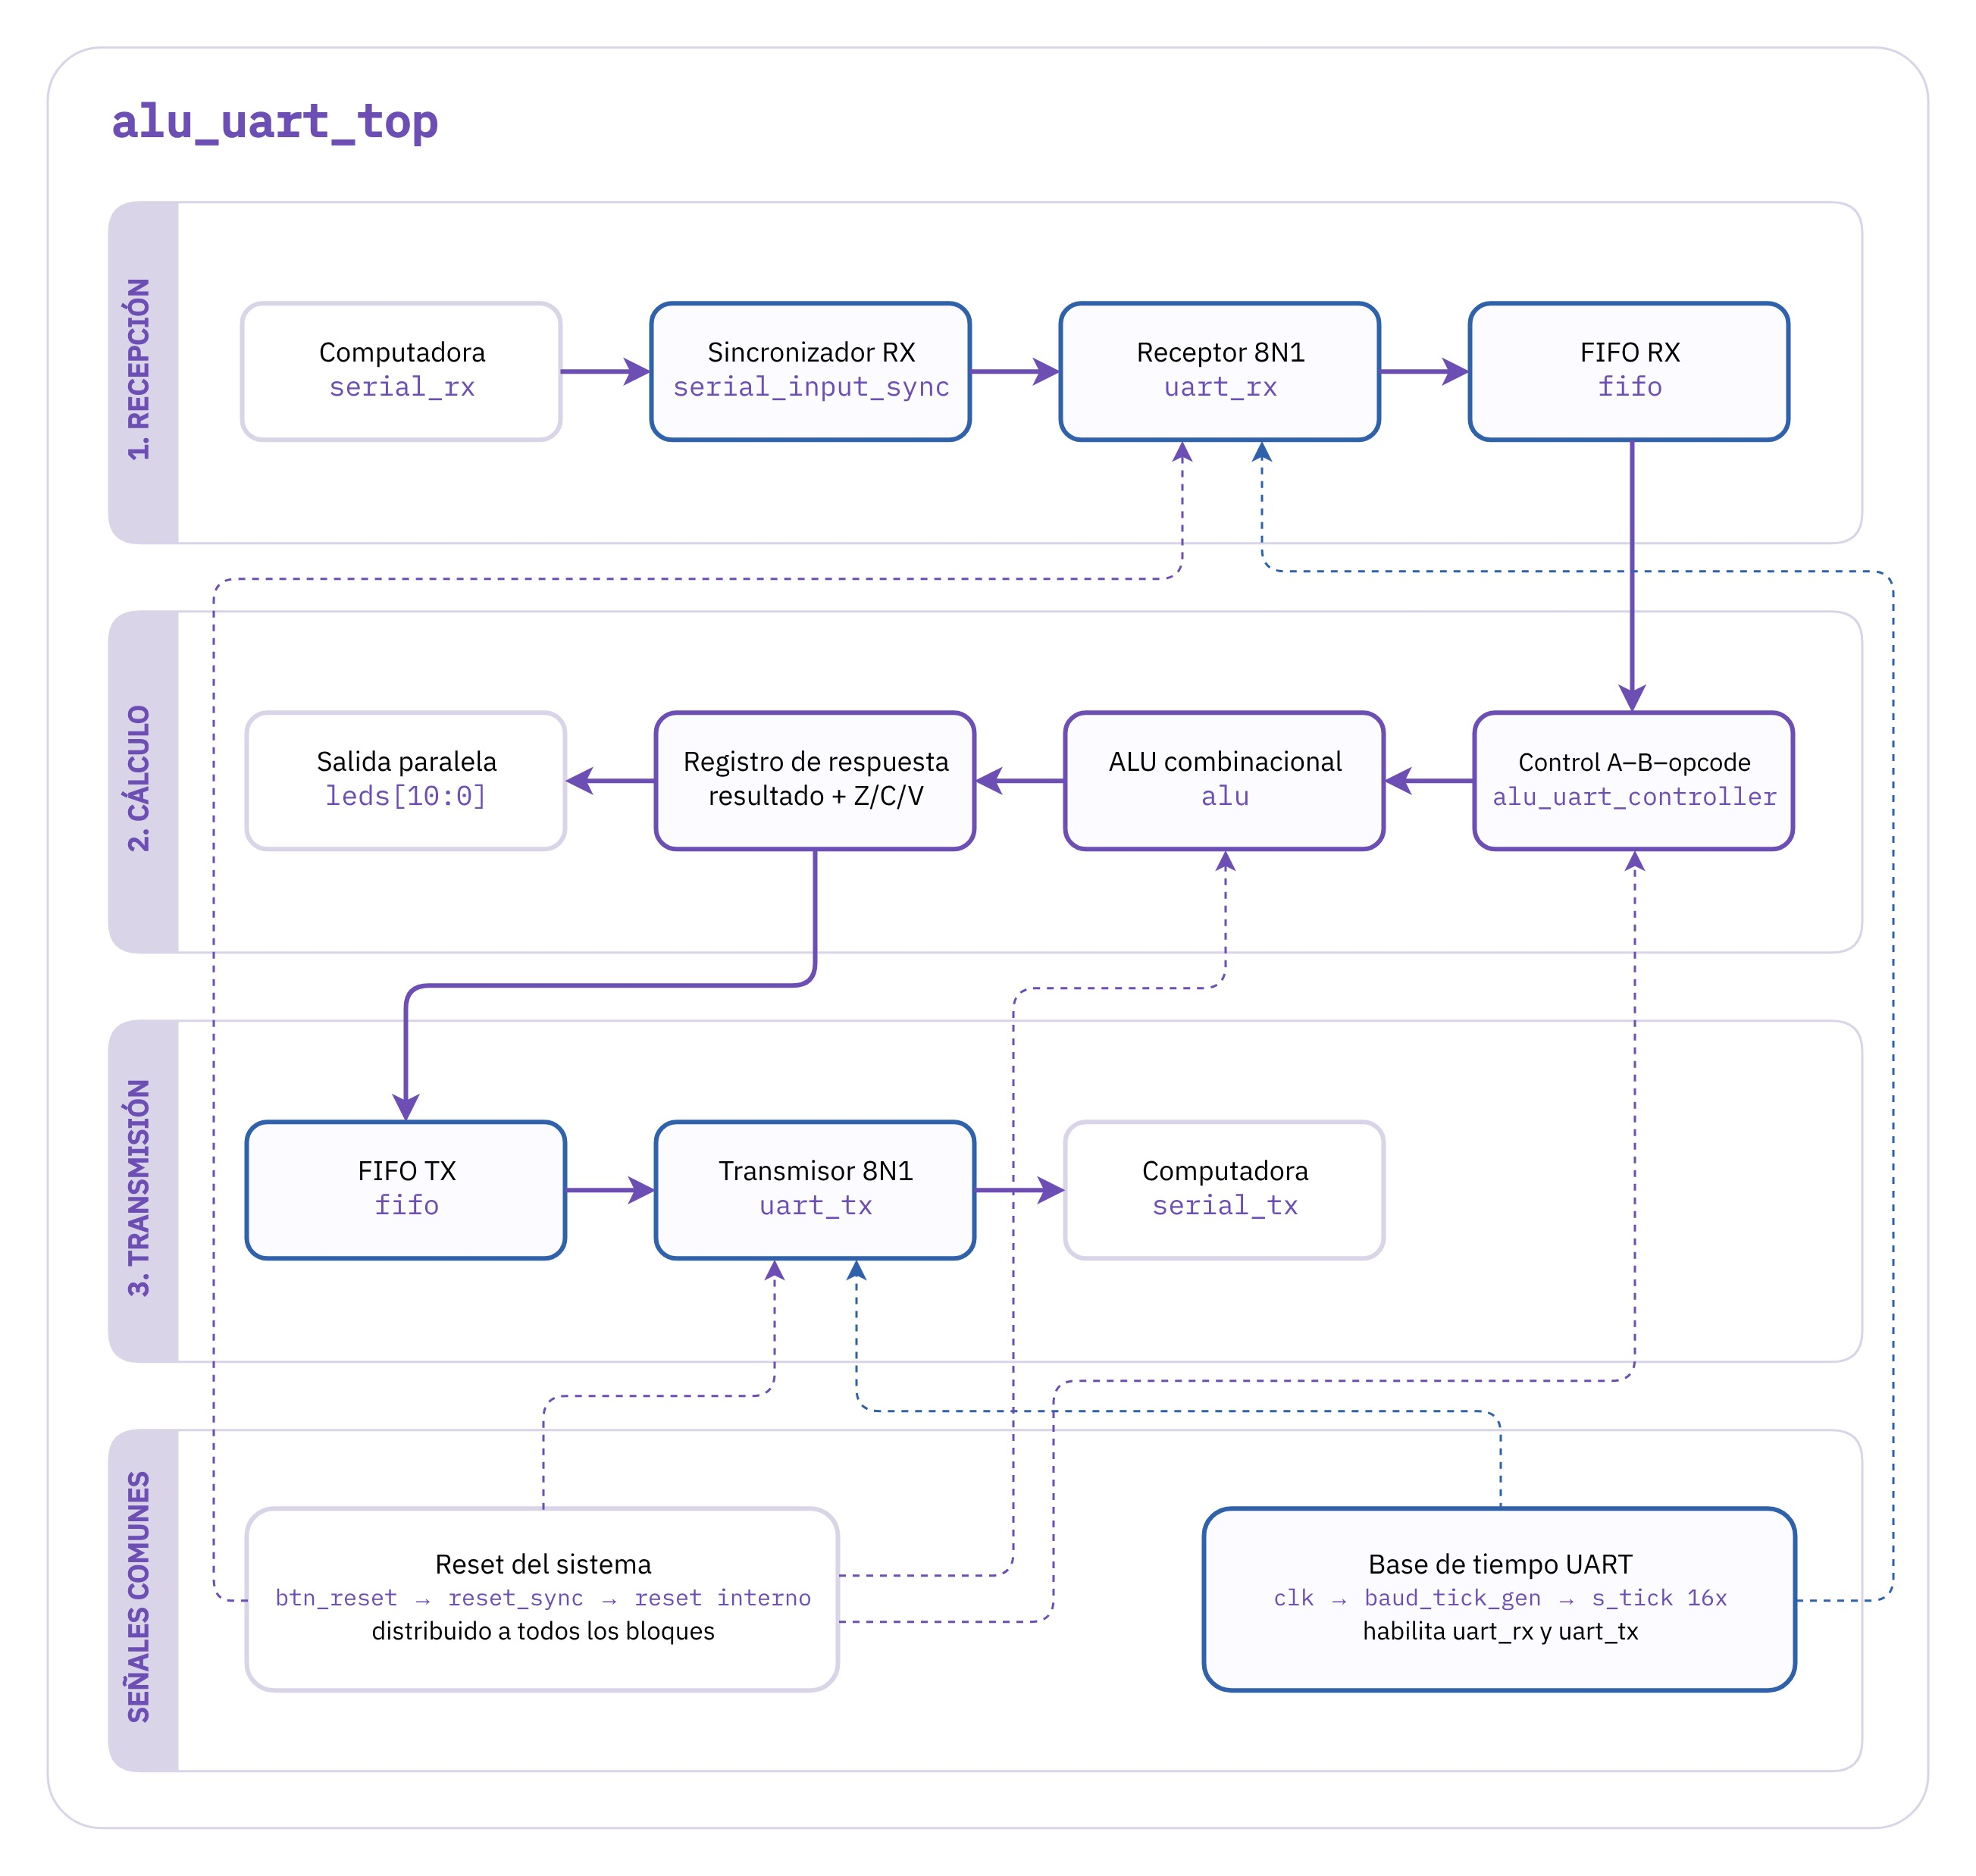
\includegraphics[width=0.88\textwidth]{img/architecture.jpg}
 \caption{Recorrido de los datos y separación funcional de la arquitectura.}%
 \label{fig:arquitectura-general}
\end{figure}

\clearpage

\newcommand{\moduleinterface}[4]{%
 \begin{figure}[H]
  \centering
  \begin{tikzpicture}[
    ifmodule/.style={draw=codeviolet,fill=codeback,rounded corners=2mm,
     minimum height=3.7cm,text width=4.5cm,align=center,thick,
    inner xsep=8pt,inner ysep=8pt,font=\normalsize},
    ifflow/.style={very thick,draw=codeviolet},
    iflabel/.style={font=\scriptsize,fill=white,inner sep=1.5pt}
   ]
   \node[ifmodule] (module) at (0,0)
   {{\color{technicalviolet}\bfseries\texttt{#1}}};
   \foreach \port/\height in {#2} {
    \draw[ifflow,-{Latex[length=2.6mm]}] (-6.6,\height) --
    node[iflabel,above] {\port} (-2.55,\height);
   }
   \foreach \port/\height in {#3} {
    \draw[ifflow,-{Latex[length=2.6mm]}] (2.55,\height) --
    node[iflabel,above] {\port} (6.6,\height);
   }
  \end{tikzpicture}
  \caption{Interfaz de #4.}%
 \end{figure}%
}

\subsection{Integración y acondicionamiento}

\texttt{alu\_uart\_top} es el módulo superior y representa el circuito conectado
a la placa. Expone únicamente el reloj de \SI{100}{\mega\hertz}, el pulsador de
reset, los pines \texttt{serial\_rx} y \texttt{serial\_tx}, y los once LED. Su
función no es procesar bits ni ejecutar operaciones: instancia los bloques
principales, les entrega los mismos parámetros de frecuencia y velocidad, y
conecta las interfaces de lectura y escritura entre el núcleo UART y el
controlador. Esta capa permite cambiar la implementación de una parte
sin alterar
los pines físicos del diseño.

\moduleinterface{alu\_uart\_top}
{{\texttt{clk}}/0.6,
 {\texttt{btn\_reset}}/0,
{\texttt{serial\_rx}}/-0.6}
{{\texttt{serial\_tx}}/0.35,
{\texttt{leds[10:0]}}/-0.35}
{\texttt{alu\_uart\_top}}

La entrada, al ser externa, puede cambiar sin relación con el reloj.
\texttt{reset\_sync} es el módulo que sincroniza ese cambio. Al
presionar el botón de reset, el reset interno se activa de inmediato;
al soltarlo, se mantiene activo durante dos flancos y recién entonces
se libera. De ese modo todos los módulos abandonan el reset sobre un
flanco conocido.

\moduleinterface{reset\_sync}
{{\texttt{clk}}/0.35,
{\texttt{async\_reset}}/-0.35}
{{\texttt{reset}}/0}
{\texttt{reset\_sync}}

\texttt{uart\_core} se ocupa de la comunicación serie. A partir de los bits que
llegan por \texttt{serial\_rx}, reconstruye cada byte y lo conserva hasta que el
controlador lo retira. En el sentido opuesto, recibe los bytes producidos por el
controlador y los transmite por \texttt{serial\_tx}.

De este modo, el controlador trabaja únicamente con bytes completos. Las señales
\texttt{rx\_empty} y \texttt{tx\_full} indican cuándo puede leer o escribir,
mientras que un pulso separado informa la recepción de una trama inválida. Los
detalles propios de UART, como la duración y el orden de los bits o la
comprobación del bit de stop, permanecen contenidos dentro del núcleo.

\moduleinterface{uart\_core}
{{\texttt{clk}}/1.35,
 {\texttt{reset}}/0.81,
 {\texttt{serial\_rx}}/0.27,
 {\texttt{rd\_uart}}/-0.27,
 {\texttt{w\_data[7:0]}}/-0.81,
{\texttt{wr\_uart}}/-1.35}
{{\texttt{serial\_tx}}/1.08,
 {\texttt{r\_data[7:0]}}/0.54,
 {\texttt{rx\_empty}}/0,
 {\texttt{tx\_full}}/-0.54,
{\texttt{rx\_error\_tick}}/-1.08}
{\texttt{uart\_core}}

\subsection{Camino de recepción}

\texttt{serial\_input\_sync} adapta la entrada asíncrona
\texttt{serial\_rx} al reloj interno. Para ello hace pasar la señal por dos
flip-flops consecutivos y utiliza solamente la salida del segundo, lo que reduce
el riesgo de propagar metastabilidad. La salida sigue siendo un único bit, que
luego es procesado por la FSM receptora.

\moduleinterface{serial\_input\_sync}
{{\texttt{clk}}/0.6,
 {\texttt{reset}}/0,
{\texttt{serial\_async}}/-0.6}
{{\texttt{serial\_sync}}/0}
{\texttt{serial\_input\_sync}}

\texttt{baud\_tick\_gen} divide el reloj del sistema y produce
\texttt{s\_tick}, una habilitación de un ciclo a dieciséis veces la velocidad de
baud. No crea un reloj nuevo. RX y TX conservan el reloj de
\SI{100}{\mega\hertz}
y solo avanzan sus contadores cuando reciben ese pulso. Compartir el generador
mantiene una única referencia temporal para ambos sentidos de la comunicación.

\moduleinterface{baud\_tick\_gen}
{{\texttt{clk}}/0.35,
{\texttt{reset}}/-0.35}
{{\texttt{s\_tick}}/0}
{\texttt{baud\_tick\_gen}}

\texttt{uart\_rx} es el receptor del enlace UART. Su función es convertir la
secuencia recibida por la línea serie en bytes de ocho bits. Cuando completa una
trama 8N1 válida, coloca el byte en
\texttt{data\_out} y activa \texttt{rx\_done\_tick} durante un ciclo.
Si la trama
es inválida, descarta el dato y lo informa mediante
\texttt{frame\_error\_tick}. De este modo, los bloques siguientes reciben bytes
completos y una indicación explícita de éxito o error.

\moduleinterface{uart\_rx}
{{\texttt{clk}}/0.9,
 {\texttt{reset}}/0.3,
 {\texttt{rx}}/-0.3,
{\texttt{s\_tick}}/-0.9}
{{\texttt{data\_out[7:0]}}/0.6,
 {\texttt{rx\_done\_tick}}/0,
{\texttt{frame\_error\_tick}}/-0.6}
{\texttt{uart\_rx}}

\texttt{rx\_fifo} es la cola de recepción. Su función es conservar los bytes
entregados por \texttt{uart\_rx} hasta que el controlador pueda procesarlos. El
byte más antiguo queda disponible en \texttt{r\_data};
\texttt{rx\_empty} indica si la cola está vacía y \texttt{rd\_uart} retira el
dato leído. Si se recibe un byte cuando no queda espacio, \texttt{uart\_core}
informa el desbordamiento mediante \texttt{rx\_error\_tick}. Esta cola y la de
transmisión son dos instancias del mismo módulo paramétrico \texttt{fifo}.

\moduleinterface{fifo}
{{\texttt{clk}}/1.2,
 {\texttt{reset}}/0.6,
 {\texttt{rd}}/0,
 {\texttt{wr}}/-0.6,
{\texttt{write\_data[7:0]}}/-1.2}
{{\texttt{read\_data[7:0]}}/0.6,
 {\texttt{empty}}/0,
{\texttt{full}}/-0.6}
{la instancia \texttt{rx\_fifo}}

\subsection{Interpretación y cálculo}

\texttt{alu\_uart\_controller} es el módulo que interpreta el protocolo de la
aplicación y coordina la ejecución de la ALU. Recibe bytes completos desde
\texttt{uart\_core}, los organiza como operando A, operando B y
opcode, y entrega
el resultado al camino de transmisión. También conserva el resultado y las
banderas que se muestran en los LED. Si ocurre un error de recepción o vence el
timeout antes de completar una solicitud, descarta los datos parciales y espera
una transacción nueva.

\moduleinterface{alu\_uart\_controller}
{{\texttt{clk}}/1.35,
 {\texttt{reset}}/0.81,
 {\texttt{r\_data[7:0]}}/0.27,
 {\texttt{rx\_empty}}/-0.27,
 {\texttt{rx\_error\_tick}}/-0.81,
{\texttt{tx\_full}}/-1.35}
{{\texttt{rd\_uart}}/0.9,
 {\texttt{w\_data[7:0]}}/0.3,
 {\texttt{wr\_uart}}/-0.3,
{\texttt{leds[10:0]}}/-0.9}
{\texttt{alu\_uart\_controller}}

\texttt{alu} es el bloque combinacional que realiza las operaciones aritméticas
y lógicas. Recibe los operandos A y B junto con los seis bits del opcode, y
produce el resultado y las banderas zero, carry y overflow. El controlador
registra esas salidas para mantenerlas estables durante la transmisión y en los
LED. De este modo, la ALU se ocupa únicamente del cálculo y no interviene en la
comunicación UART.

\moduleinterface{alu}
{{\texttt{i\_data\_a[7:0]}}/0.6,
 {\texttt{i\_data\_b[7:0]}}/0,
{\texttt{i\_data\_opcode[5:0]}}/-0.6}
{{\texttt{o\_result[7:0]}}/0.9,
 {\texttt{o\_zero}}/0.3,
 {\texttt{o\_carry}}/-0.3,
{\texttt{o\_overflow}}/-0.9}
{\texttt{alu}}

\subsection{Camino de transmisión y salidas}

\texttt{tx\_fifo} es la cola de transmisión. Almacena los bytes producidos por
el controlador hasta que \texttt{uart\_tx} pueda enviarlos. El controlador
escribe mediante \texttt{w\_data} y \texttt{wr\_uart}, mientras que
\texttt{tx\_full} indica si existe espacio disponible. Cuando la cola está
llena, el controlador conserva el resultado y espera, evitando que se pierda la
respuesta.

\moduleinterface{fifo}
{{\texttt{clk}}/1.2,
 {\texttt{reset}}/0.6,
 {\texttt{rd}}/0,
 {\texttt{wr}}/-0.6,
{\texttt{write\_data[7:0]}}/-1.2}
{{\texttt{read\_data[7:0]}}/0.6,
 {\texttt{empty}}/0,
{\texttt{full}}/-0.6}
{la instancia \texttt{tx\_fifo}}

\texttt{uart\_tx} es el transmisor del enlace UART. Su función es convertir un
byte completo en una trama 8N1 y enviarla por la salida serie. La señal
\texttt{tx\_start} inicia la transmisión, \texttt{tx\_busy} indica que el módulo
está ocupado y \texttt{tx\_done\_tick} informa que la trama terminó. La salida
\texttt{tx} se conecta a \texttt{serial\_tx} en el nivel superior.

\moduleinterface{uart\_tx}
{{\texttt{clk}}/1.2,
 {\texttt{reset}}/0.6,
 {\texttt{tx\_start}}/0,
 {\texttt{s\_tick}}/-0.6,
{\texttt{data\_in[7:0]}}/-1.2}
{{\texttt{tx}}/0.6,
 {\texttt{tx\_done\_tick}}/0,
{\texttt{tx\_busy}}/-0.6}
{\texttt{uart\_tx}}

Los once LED se controlan de forma independiente al transmisor. Muestran el
resultado registrado y las banderas Z, C y V, por lo que conservan su estado
aunque la respuesta UART ya haya finalizado.

Esta distribución establece una regla clara entre módulos: el productor solo
escribe si la cola no está llena y el consumidor solo lee si no está vacía. Las
señales \texttt{wr}/\texttt{full} y \texttt{rd}/\texttt{empty} convierten una
relación temporal implícita en un contrato verificable. Gracias a ello, cada
bloque puede probarse de manera aislada antes de comprobar el
recorrido completo.

\section{Flujo de operación}

En reposo, las señales RX y TX permanecen en nivel alto, la cola de
recepción se encuentra vacía y el controlador espera el operando A.
Cuando llega una trama válida, RX entrega el byte recibido a la cola
de recepción. El controlador lo retira y pasa a esperar el operando
B; el proceso se repite para el opcode. En el estado correspondiente
la ALU ve los tres registros estables. Un ciclo después se capturan
el resultado y las banderas, y se espera a que haya capacidad
suficiente en la cola del transmisor.

La respuesta no se retira de la cola de transmisión cuando comienza a
transmitirse, sino al final del stop. En consecuencia, el dato
frontal permanece estable durante toda la trama. Si llega un error
antes de recibir los tres operandos, el controlador descarta los
registros parciales y el próximo byte vuelve a interpretarse como el
operando A. Esta regla evita asociar datos pertenecientes a
solicitudes distintas.

\section{Decisiones de diseño}

El protocolo con la computadora se mantuvo deliberadamente pequeño. Cada
solicitud está formada por tres bytes binarios enviados en un orden
fijo: primero
el operando A, después el operando B y por último el código de
operación. Una vez
recibida la terna, el circuito responde con un único byte de resultado. Este
formato evita incorporar un analizador de texto, conversiones desde ASCII o
caracteres separadores, recursos que no contribuirían al objetivo del trabajo.
Como contrapartida, el emisor debe respetar el orden acordado y el controlador
debe recordar cuántos bytes válidos recibió antes de ejecutar la ALU.

La UART opera a \num{19200} baud, una velocidad muy inferior al reloj de
\SI{100}{\mega\hertz} de la placa. Para relacionar ambas velocidades,
\texttt{baud\_tick\_gen} cuenta ciclos del reloj principal y activa
\texttt{s\_tick} cada 326 ciclos. De esta forma se obtienen aproximadamente
dieciséis instantes de referencia durante cada bit de la trama UART.

El receptor y el transmisor continúan sincronizados con el reloj de
\SI{100}{\mega\hertz}, pero utilizan \texttt{s\_tick} para determinar cuándo
avanzar. Por lo tanto, \texttt{s\_tick} es una señal de habilitación y no un
segundo reloj. El receptor aprovecha esas referencias para verificar el inicio
de la trama y leer cada bit cerca de su centro.

La recepción, la transmisión y la interpretación de una solicitud avanzan por
etapas y deben recordar cuál es la siguiente acción. Por eso cada una se
controla mediante una máquina de estados: RX, TX y el controlador. Las tres
utilizan codificación one-hot. Cada estado posee su propio flip-flop: RX emplea
cinco, TX cuatro y el controlador otros cinco. Frente
a una codificación binaria se consumen más registros, pero en esta FPGA el costo
es reducido y se obtiene una relación directa entre cada estado y su bit de
representación. Esto simplifica el seguimiento de las transiciones durante la
simulación y permite reconocer con facilidad el estado activo en los reportes de
síntesis. El atributo \texttt{fsm\_encoding = "one\_hot"} deja explícita esa
elección, y la rama por defecto de cada FSM define además un retorno
seguro si el
registro de estado adopta una combinación inválida.

Los FIFO resuelven la diferencia de ritmo entre la comunicación UART y el
procesamiento interno. Se eligió una profundidad de cuatro bytes porque alcanza
para absorber una ráfaga breve sin convertir las colas en memoria
para una sesión
completa. En recepción, cada trama válida ocupa una posición hasta que el
controlador la retira; si llega un nuevo byte con las cuatro
posiciones ocupadas,
el núcleo no sobrescribe información previa y notifica el desbordamiento
(\textit{overrun}). En
transmisión, la situación se resuelve mediante espera: si \texttt{tx\_full} está
activo, el controlador conserva el resultado y sus banderas hasta que exista una
posición libre. El registro de respuesta también mantiene estables los LED y
evita que una solicitud parcial modifique el último resultado válido.

El orden fijo de tres bytes plantea un último problema: si la computadora envía
A o A--B y luego interrumpe la transferencia, el controlador no puede conservar
esa solicitud incompleta de manera indefinida. Por ese motivo se incorporó un
tiempo máximo de espera (\textit{timeout}) de \SI{10}{\milli\second}. A
\num{19200} baud, una trama 8N1 dura
aproximadamente \SI{0.521}{\milli\second}, de modo que el margen admite pausas
considerablemente mayores que el tiempo de transmisión normal. Si el plazo vence
o RX informa un error antes de completar la terna, se descartan los registros
parciales y el siguiente byte vuelve a interpretarse como el operando A.

En conjunto, estas decisiones priorizan un comportamiento determinista y
verificable. Cada bloque posee una condición explícita para aceptar datos,
esperar o recuperarse, sin depender de retardos implícitos entre módulos.

\section{Organización del proyecto}

El árbol de la figura~\ref{fig:jerarquia-modulos} refleja la jerarquía
sintetizable, no solo la distribución de archivos.\ \texttt{alu\_uart\_top}
instancia el acondicionador de reset, el núcleo UART y el
controlador. Dentro del
núcleo quedan sincronizador, generador, receptor, transmisor y ambos
FIFO; dentro
del controlador se conserva la ALU del TP1.

\begin{figure}[H]
 \centering
 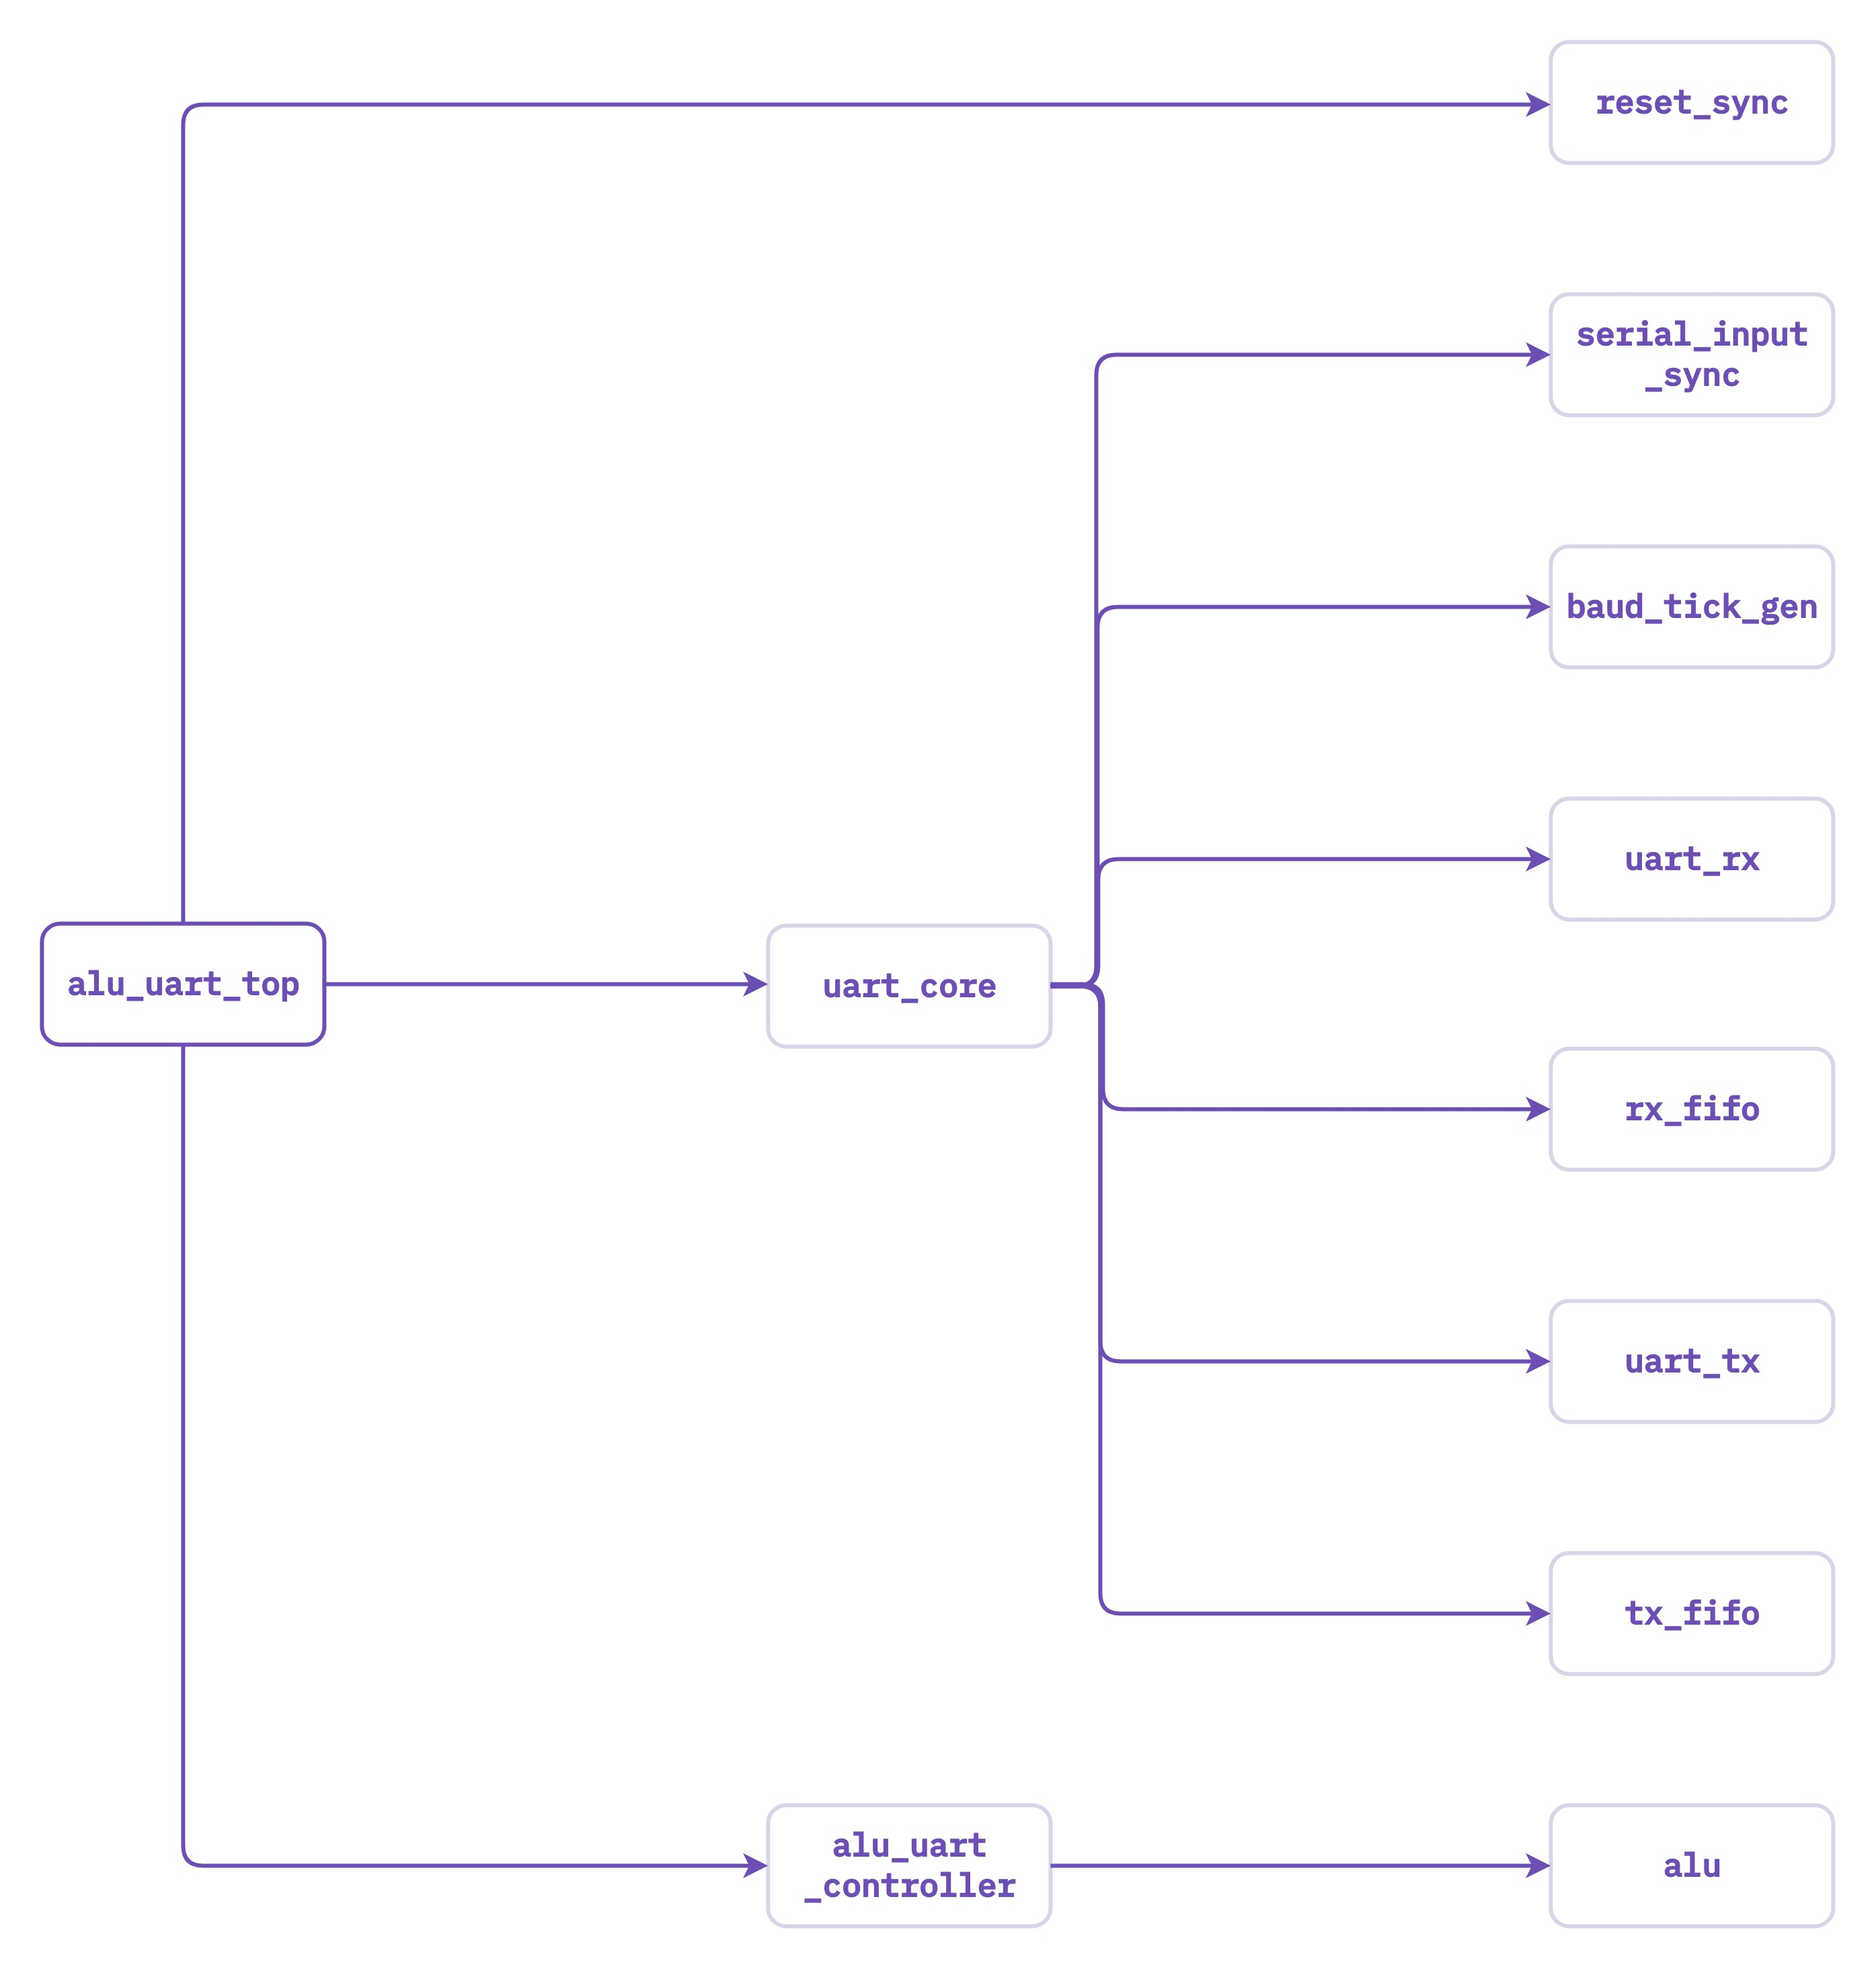
\includegraphics[height=10.8cm,keepaspectratio]{img/modules.jpg}
 \caption{Jerarquía de módulos elaborada a partir de las instancias RTL.}%
 \label{fig:jerarquia-modulos}
\end{figure}
